
\chapter{Vérification annuelle}
\label{chap:verification}

\section{Objectifs}

La vérification annuelle permet au fournisseur de comparer les consommations enregistrées mensuellement pour chaque client avec les relevés annuels transmis par l'agent.

Cette opération vise principalement à :
\begin{itemize}
    \item calculer la consommation annuelle à partir des relevés mensuels validés ou facturés ;
    \item comparer les résultats obtenus avec les valeurs du relevé annuel de l'agent ;
    \item identifier les écarts dépassant une tolérance définie ;
    \item permettre au fournisseur de valider ou de rejeter le relevé annuel ;
    \item informer le client de la décision prise.
\end{itemize}

\section{Consommations mensuelles}

La vérification s'appuie sur les enregistrements de la table \texttt{consommation}. Seules les consommations dont le statut est \texttt{VALIDEE} ou \texttt{FACTUREE} sont prises en compte.

Pour chaque client et pour l'année sélectionnée, le système récupère :
\begin{itemize}
    \item les relevés mensuels validés ou facturés ;
    \item les index d'eau et d'électricité ;
    \item les informations permettant de distinguer les différents contrats du client.
\end{itemize}

Le nombre de relevés retenus est également calculé. Le système utilise une constante de douze relevés attendus pour l'année.

\textbf{Remarque :} dans l'implémentation actuelle, ce nombre correspond au nombre d'enregistrements de consommation retenus, et non au nombre de mois distincts. Un client possédant plusieurs contrats peut donc avoir plusieurs relevés pour un même mois.

\section{Relevé annuel de l'Agent}

Les relevés annuels sont enregistrés dans la table \texttt{conso\_annuelle}. Chaque enregistrement contient notamment :
\begin{itemize}
    \item l'identifiant du client ;
    \item l'identifiant de l'agent ayant effectué le relevé ;
    \item la consommation annuelle d'eau ;
    \item la consommation annuelle d'électricité ;
    \item l'année concernée ;
    \item la date de saisie ;
    \item le statut de vérification et la date de décision.
\end{itemize}

La base de données impose une contrainte d'unicité sur le couple \texttt{(id\_client, annee)}. Ainsi, un seul relevé annuel est conservé pour un client et une année.

La page de vérification récupère les relevés annuels disponibles pour les clients du fournisseur connecté. Lorsqu'un relevé existe, ses consommations sont affichées en regard des consommations calculées à partir des relevés mensuels.

\section{Calcul par contrat}

Un même client peut posséder plusieurs contrats. Le calcul annuel doit donc tenir compte de chaque contrat séparément avant d'additionner les résultats.

Pour chaque contrat, le système recherche :
\begin{itemize}
    \item le dernier index validé ou facturé avant l'année sélectionnée ;
    \item le dernier index validé ou facturé pendant l'année sélectionnée.
\end{itemize}

La consommation annuelle d'un contrat est calculée par différence entre ces deux index :

\[
C_{\text{annuelle}} =
\max(0, I_{\text{fin}} - I_{\text{base}})
\]

où :
\begin{itemize}
    \item \(I_{\text{fin}}\) représente le dernier index de l'année ;
    \item \(I_{\text{base}}\) représente le dernier index antérieur à l'année.
\end{itemize}

Si aucun index antérieur n'est disponible, le système utilise zéro comme index de base.

Les consommations calculées pour les différents contrats sont ensuite additionnées afin d'obtenir les consommations annuelles du client :

\[
C_{\text{client}} =
\sum_{i=1}^{n} C_{\text{contrat}_i}
\]

Ce calcul est effectué séparément pour l'eau et l'électricité.

\section{Tolérance}

Le système utilise une tolérance maximale de \(5\,\%\) pour comparer la consommation calculée à partir des relevés mensuels avec celle déclarée par l'agent.

L'écart relatif est calculé à l'aide de la formule suivante :

\[
E(\%) =
\frac{|C_{\text{saisie}} - C_{\text{agent}}|}
{C_{\text{agent}}}
\times 100
\]

où :
\begin{itemize}
    \item \(C_{\text{saisie}}\) désigne la consommation calculée à partir des relevés mensuels ;
    \item \(C_{\text{agent}}\) désigne la consommation annuelle relevée par l'agent.
\end{itemize}

Lorsque la consommation de l'agent est nulle, le système considère l'écart comme égal à \(100\,\%\) si la consommation calculée est positive, et à \(0\,\%\) dans le cas contraire.

Le résultat de l'analyse est déterminé selon les règles suivantes :
\begin{itemize}
    \item \textbf{Sans relevé :} aucun relevé annuel de l'agent n'est disponible ;
    \item \textbf{Incomplet :} le nombre de relevés mensuels enregistrés est inférieur à douze ;
    \item \textbf{Écart :} l'écart calculé pour l'eau ou l'électricité dépasse \(5\,\%\) ;
    \item \textbf{Conforme :} les conditions précédentes ne sont pas réunies.
\end{itemize}

Un écart égal à \(5\,\%\) reste donc dans la tolérance. Le résultat est considéré comme un écart uniquement lorsque la valeur dépasse ce seuil.

\section{Interface fournisseur}

L'interface de vérification est accessible au fournisseur connecté. Elle présente les clients associés à ce fournisseur et les informations nécessaires à la comparaison annuelle.

Un filtre permet de sélectionner l'année à examiner. Par défaut, le système privilégie la dernière année pour laquelle un relevé annuel de l'agent est disponible, ou l'année proposée par la liste lorsque ce relevé n'existe pas.

Pour chaque client, le tableau affiche :
\begin{itemize}
    \item le nom, le prénom et le CIN ;
    \item le nombre de relevés mensuels enregistrés ;
    \item la consommation annuelle d'eau calculée et celle de l'agent ;
    \item l'écart relatif pour l'eau ;
    \item la consommation annuelle d'électricité calculée et celle de l'agent ;
    \item l'écart relatif pour l'électricité ;
    \item le résultat de l'analyse ;
    \item le statut de la décision du fournisseur.
\end{itemize}

Les résultats sont différenciés visuellement à l'aide de badges : conforme, écart à vérifier, saisie incomplète ou relevé agent absent.

\section{Validation et rejet}

Lorsqu'un relevé annuel de l'agent existe, le fournisseur dispose de deux actions :
\begin{itemize}
    \item \textbf{Valider :} enregistrer la décision \texttt{VALIDEE} ;
    \item \textbf{Rejeter :} enregistrer la décision \texttt{REJETEE}.
\end{itemize}

La décision est transmise par une requête POST. Le traitement vérifie le jeton CSRF, le rôle du fournisseur, l'identifiant du client, l'année et la valeur de la décision.

La requête de mise à jour vérifie également que le client appartient bien au fournisseur connecté. Le statut de vérification ainsi que la date de décision sont ensuite enregistrés dans la table \texttt{conso\_annuelle}.

Dans l'implémentation actuelle, la validation ou le rejet reste possible dès lors qu'un relevé annuel existe, même si l'analyse indique un écart ou une saisie incomplète. Le résultat de l'analyse constitue donc une aide à la décision et ne bloque pas automatiquement les actions du fournisseur.

\section{Notification client}

Après l'enregistrement d'une décision, le système tente de créer une notification destinée au client concerné.

Le message dépend de la décision :
\begin{itemize}
    \item après une validation, le client est informé que sa consommation annuelle a été validée ;
    \item après un rejet, le client est informé qu'un écart a été constaté et qu'il doit contacter le fournisseur.
\end{itemize}

La notification est enregistrée avec le type \texttt{VERIFICATION} et contient un lien vers la page des consommations du client.

Si la création de la notification échoue, l'erreur est enregistrée dans le journal technique. Cette situation n'annule pas la décision déjà enregistrée.

\section{Tests}

Les scénarios suivants permettent de vérifier le fonctionnement du module :
\begin{itemize}
    \item vérifier l'affichage des clients associés au fournisseur connecté ;
    \item sélectionner une année et vérifier le chargement des données correspondantes ;
    \item vérifier le calcul annuel d'un client possédant un seul contrat ;
    \item vérifier l'addition des consommations lorsque le client possède plusieurs contrats ;
    \item vérifier le résultat lorsque les douze relevés attendus ne sont pas disponibles ;
    \item vérifier le résultat lorsque l'écart est inférieur, égal ou supérieur à \(5\,\%\) ;
    \item vérifier le cas où aucun relevé annuel de l'agent n'existe ;
    \item vérifier l'enregistrement d'une décision de validation ou de rejet ;
    \item vérifier que le fournisseur ne peut pas décider pour un client appartenant à un autre fournisseur ;
    \item vérifier la création de la notification destinée au client après la décision.
\end{itemize}

Ces scénarios constituent les vérifications fonctionnelles à effectuer sur le module.

\begin{figure}[H]
  \centering
  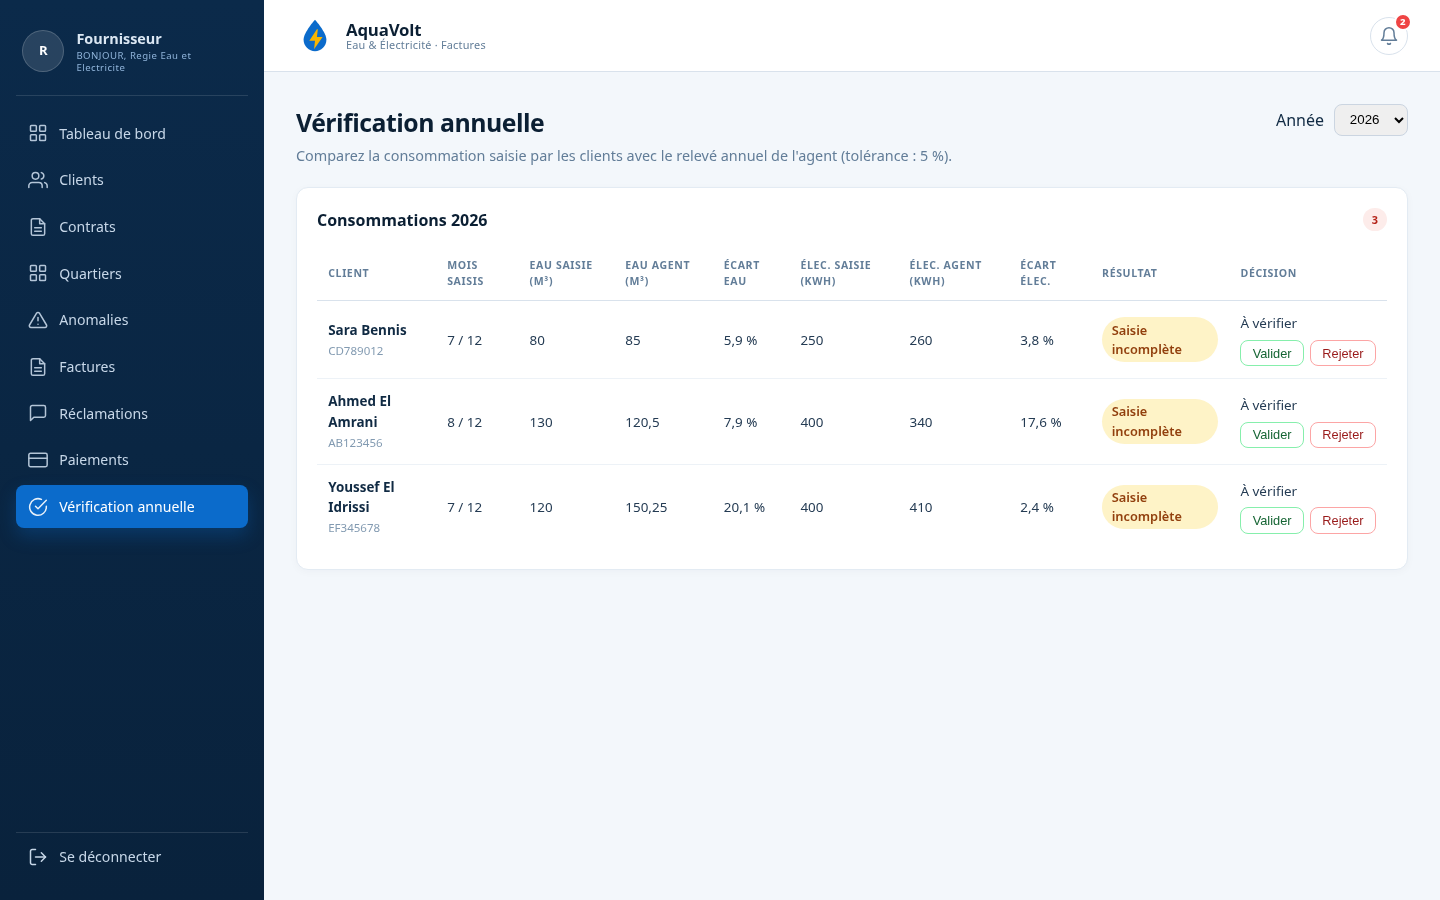
\includegraphics[width=0.95\textwidth]{../tests/final/desktop/10_verification_page.png}
  \caption{Vérification annuelle des consommations}
  \label{fig:verification}
\end{figure}
